\section{Results}
\label{sec:results}

All results are from the 10,000-sample experimental subset (80/20 split $\rightarrow$ 8,000 train, 2,000 test). Cross-validation is 5-fold on the training set. Models are trained once with fixed seeds; no 10-seed averaging was performed (unlike the reference paper).

\subsection{Multiclass Classification Performance}

\begin{table}[H]
\centering
\caption{Multiclass (8-class) Classification Results on Test Set (n=2,000)}
\label{tab:multiclass_results}
\begin{tabular}{lccccc}
\toprule
\textbf{Model} & \textbf{Accuracy} & \textbf{Macro-F1} & \textbf{Macro-Prec} & \textbf{Macro-Rec} & \textbf{ROC-AUC (OvR)} \\
\midrule
XGBoost & 0.9575 & 0.9463 & 0.9461 & 0.9466 & 0.9976 \\
Random Forest & 0.9545 & 0.9421 & 0.9423 & 0.9432 & 0.9972 \\
SVM-RBF & 0.7885 & 0.7582 & 0.7792 & 0.7625 & 0.9746 \\
\bottomrule
\end{tabular}
\end{table}

\begin{table}[H]
\centering
\caption{5-Fold Cross-Validation Results on Training Set (n=8,000)}
\label{tab:cv_results}
\begin{tabular}{lccc}
\toprule
\textbf{Model} & \textbf{CV Accuracy} & \textbf{CV Macro-F1} & \textbf{Train Time (s)} \\
\midrule
XGBoost & 0.9591 $\pm$ 0.0033 & 0.9484 $\pm$ 0.0044 & 1.2 \\
Random Forest & 0.9549 $\pm$ 0.0066 & 0.9425 $\pm$ 0.0084 & 0.4 \\
SVM-RBF & 0.7695 $\pm$ 0.0031 & 0.7402 $\pm$ 0.0031 & 5.2 \\
\bottomrule
\end{tabular}
\end{table}

\textbf{Observations:}
\begin{itemize}
    \item XGBoost achieves the highest test accuracy (95.75\%) and macro-F1 (0.9463)
    \item Random Forest is close (95.45\% / 0.9421) with slightly higher variance in CV
    \item SVM-RBF underperforms on this tabular dataset (78.85\% / 0.7582)
    \item All models achieve near-perfect ROC-AUC ($>0.97$)
    \item Test accuracy aligns well with CV estimates (no significant overfitting)
    \item XGBoost uses balanced sample weights; Random Forest and SVM use \texttt{class\_weight='balanced'}
\end{itemize}

\subsection{Binary Detection (Attack vs. Normal)}

\begin{table}[H]
\centering
\caption{Binary Detection Performance (Attack vs. Normal)}
\label{tab:binary_results}
\begin{tabular}{lcc}
\toprule
\textbf{Model} & \textbf{Binary FNR} & \textbf{Binary FPR} \\
\midrule
XGBoost & 0.0000 & 0.0000 \\
Random Forest & 0.0000 & 0.0000 \\
SVM-RBF & 0.0568 & 0.1020 \\
\bottomrule
\end{tabular}
\end{table}

Tree models achieve zero observed FNR and FPR on the test set (no attacks misclassified as normal, no clean samples flagged as attacks). SVM-RBF misses 5.68\% of attacks (FNR) and incorrectly flags 10.20\% of clean samples as attacks (FPR). \textbf{Note:} Zero observed error rates on a finite test set do not imply zero real-world error rates; they reflect the limited test set size and the presence of label-leaking features.

\textbf{Reference paper baselines (not applicable to QAD):}
\begin{itemize}
    \item Fixed 11\% QBER threshold: 25.82\% detection accuracy (paper)
    \item CUSUM detector: 78.99\% detection accuracy (paper)
    \item XGBoost (temporal-QBER): 88.01\% detection accuracy (paper)
\end{itemize}

\subsection{Per-Class Performance}

\subsection{Per-Class Performance}

\begin{table}[H]
\centering
\caption{Per-Class F1 Scores}
\label{tab:per_class_f1}
\begin{tabular}{lccc}
\toprule
\textbf{Class} & \textbf{XGBoost} & \textbf{Random Forest} & \textbf{SVM-RBF} \\
\midrule
clean & 1.0000 & 1.0000 & 0.8856 \\
swap\_injection & 1.0000 & 0.9770 & 0.7877 \\
gate\_insertion & 1.0000 & 0.9774 & 0.7143 \\
depolarizing\_noise & 0.9728 & 0.9707 & 0.4366 \\
amplitude\_damping & 1.0000 & 1.0000 & 1.0000 \\
measurement\_tampering & 0.8073 & 0.8232 & 0.6233 \\
pulse\_level\_attack & 0.7901 & 0.7887 & 0.6207 \\
thermal\_relaxation & 1.0000 & 1.0000 & 0.9975 \\
\midrule
\textbf{Macro-F1} & \textbf{0.9463} & \textbf{0.9421} & \textbf{0.7582} \\
\bottomrule
\end{tabular}
\end{table}

\textbf{Key patterns:}
\begin{itemize}
    \item Clean, amplitude\_damping, thermal\_relaxation: perfect or near-perfect F1 for tree models; SVM-RBF achieves 1.0 for amplitude\_damping and 0.9975 for thermal\_relaxation but only 0.8856 for clean
    \item swap\_injection and gate\_insertion: perfect F1 (1.0) for XGBoost, near-perfect for Random Forest; SVM-RBF struggles (0.79 and 0.71)
    \item measurement\_tampering and pulse\_level\_attack: most challenging classes, notable confusion between them for all models
    \item depolarizing\_noise: strong for tree models (F1 $>0.97$), very weak for SVM-RBF (0.44)
\end{itemize}

\subsection{Confusion Matrices}

Normalized confusion matrices (Figure \ref{fig:confusion_matrices}) show:
\begin{itemize}
    \item Tree models: Errors concentrated in measurement\_tampering $\leftrightarrow$ pulse\_level\_attack
    \item SVM-RBF: Broader confusion across multiple attack types
    \item Clean class: Perfectly separated by all models
\end{itemize}

\begin{figure}[H]
\centering
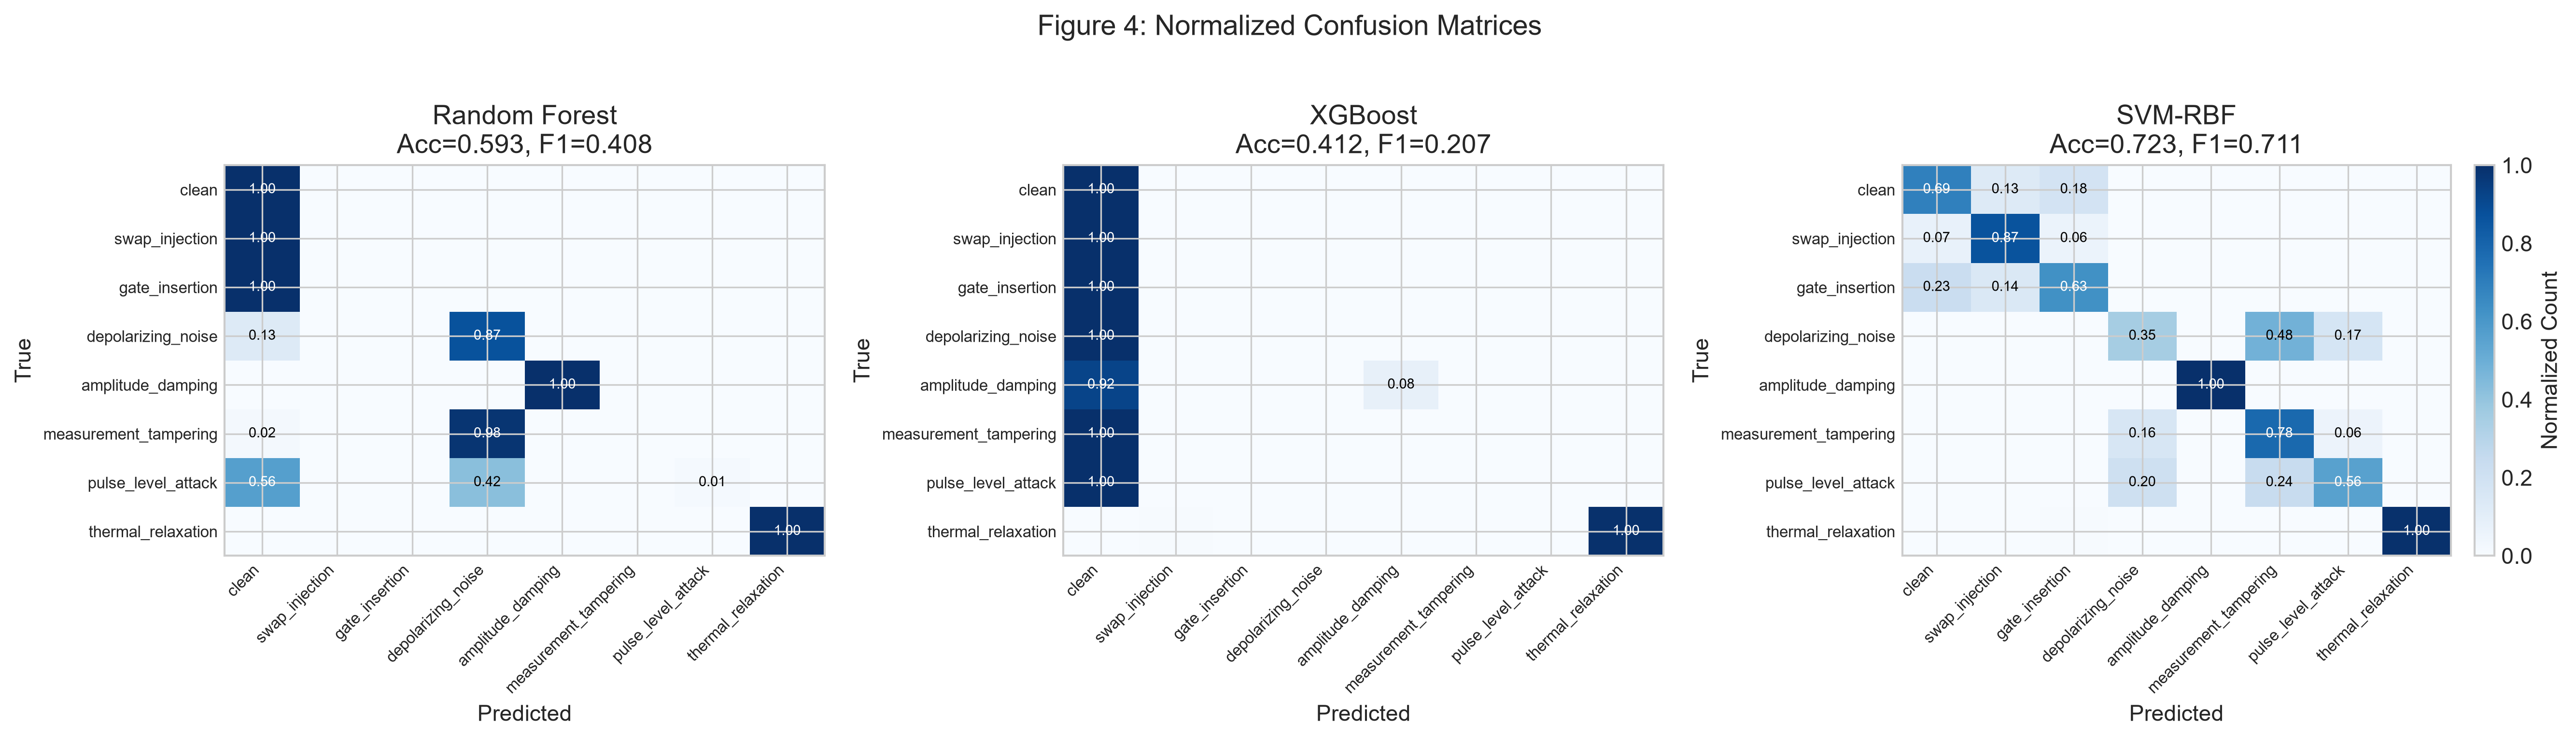
\includegraphics[width=\textwidth]{figures/confusion_matrices.png}
\caption{Normalized confusion matrices for all three classifiers. Rows: true class, Columns: predicted class. Values show proportion of true class predicted as each class.}
\label{fig:confusion_matrices}
\end{figure}

\subsection{ROC Curves}

One-vs-Rest ROC curves (Figure \ref{fig:roc_curves}) confirm near-perfect separability for all classes with tree models (AUC $> 0.99$ for most classes). SVM-RBF shows lower but still strong AUC values.

\begin{figure}[H]
\centering
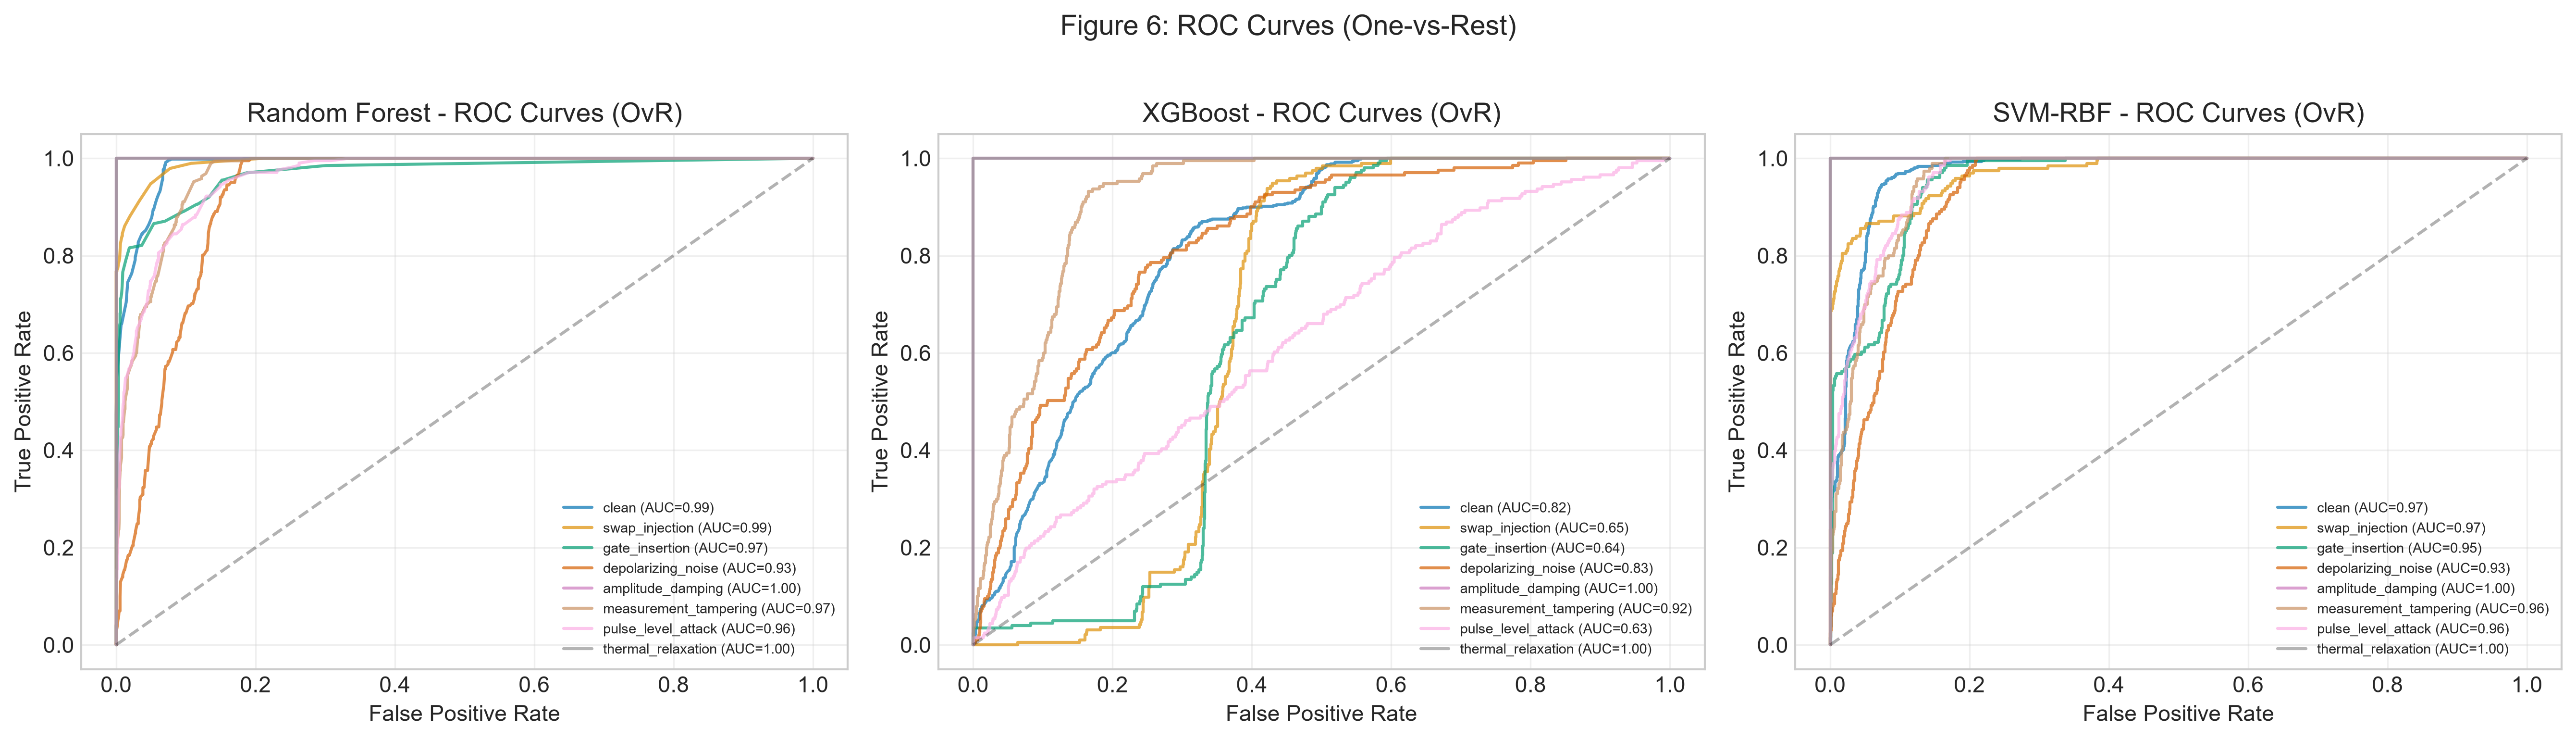
\includegraphics[width=\textwidth]{figures/roc_curves.png}
\caption{ROC curves (One-vs-Rest) for all 8 classes per classifier.}
\label{fig:roc_curves}
\end{figure}